\section{Expérience A3} 
  \subsection{Objectif}
    Comprendre de quelles manières peuvent émerger des représentations et méta-représentations dans 
    un réseau de neurone connexionniste, plus particulièrement sur des perceptrons multicouches.
    
    Réalisation de la première expérience de l'article \cite{Cleeremans_2007} sur des données réelles.
    
  \subsection{Architecture}
    \paragraph{Description}
      Un premier réseau de perceptron multicouche apprend à discrétiser des chiffres représentés
      par 256 (16x16) neurones d'entrées. Il est composé d'une couche cachée de 64 neurones.
      
      Un second réseau de perceptron multicouche apprend à dupliquer toutes les couches du premier
      réseau en n'ayant que sa couche cachée en entrée.
      
      L'apprentissage du second réseau, n'affecte pas les poids entre la couche d'entrée et la 
      couche cachée du premier réseau.

    \paragraph{Schéma}
      \begin{center}
	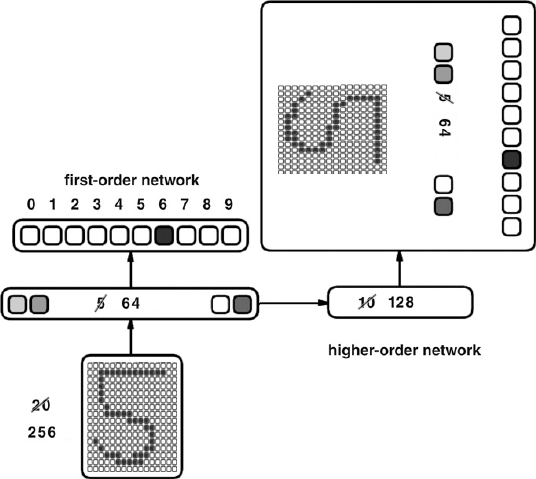
\includegraphics[width=220px]{data/expA3/schema.png}
      \end{center}
      
    \paragraph{Paramètres}
      \begin{center}
	\begin{tabular}{lr}
	  \begin{minipage}{230px}
	    \begin{itemize}
	      \item momentum : 0.9 sur les 2 réseaux
	      \item taux d'apprentissage : 0.1 sur les 2 réseaux
	      \item \textbf{1600 formes} de chiffres différents présentées (shuffle) \cite{Handwritten_256}
	      \item apprentissage 10 (formes) x 1000 (époques)
	    \end{itemize}
	  \end{minipage}
	  &
	  \begin{minipage}{230px}
	    \begin{itemize}
	      \item poids initialisés sur [-0.25 ; 0.25]
	      \item taux d'apprentissage constant
	      \item entrées valent 0 ou 1
	      \item sigmoïde à température 1
	      \item utilisation de biais
	    \end{itemize}
	  \end{minipage}
	\end{tabular}
      \end{center}

  
  \newpage
  \subsection{Résultats}
    \paragraph{Principaux}
      Analyse des performances
      \begin{center}
	\begin{tabular}{lr}
	  \hspace*{-1cm}
	  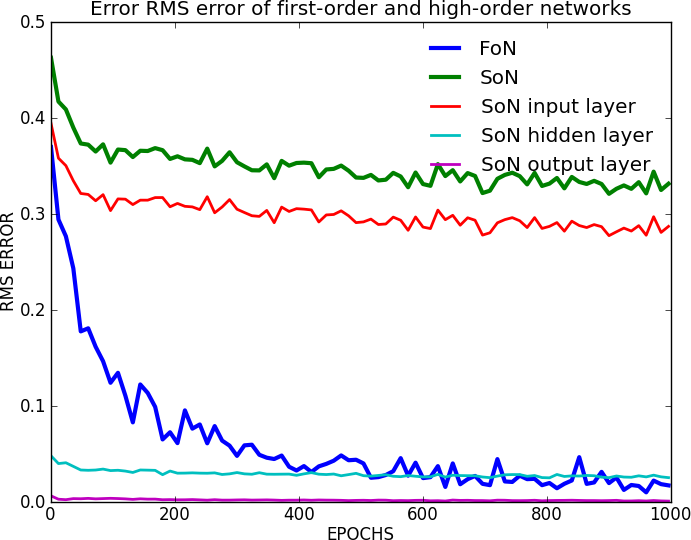
\includegraphics[width=250px]{data/expA3/rms.png}
	  &
	  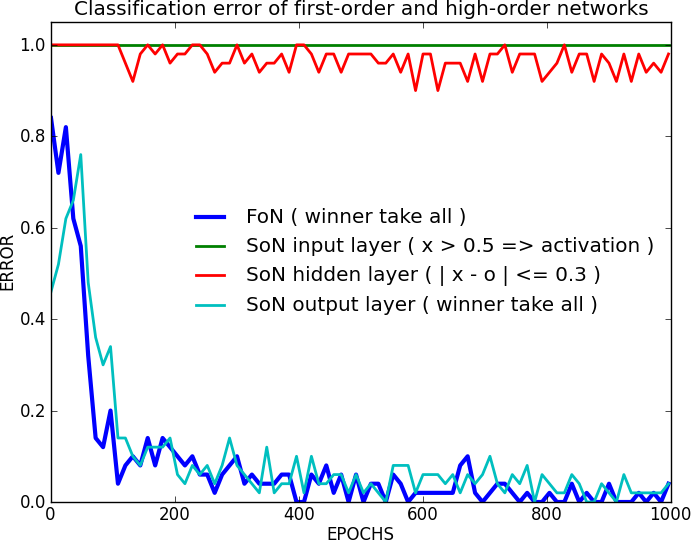
\includegraphics[width=250px]{data/expA3/err.png} 
	\end{tabular}
      \end{center}
      \subparagraph{Notes}
	\begin{itemize}
	  \item formule utilisée pour RMS (cf. Formules~\nameref{rms})
	  \item les courbes SoN layer représentent les erreurs (du second réseaux) sur les couches à reproduire 
	  \item la courbe RMS verte (SoN) est la somme des 3 courbes SoN layer
	\end{itemize}
      \subparagraph{Conclusion}
	\begin{itemize}
	  \item le premier réseau réussit à apprendre sa tâche de classification
	  \item la couche cachée et la couche de sortie posent peu de problèmes d'apprentissage
	  \item le second réseau a du mal à reproduire les entrées
	  \item le second réseau apprend maintenant (vs \nameref{expA1}, \nameref{expA2}) moins rapidement que le premier
	\end{itemize}
    \paragraph{Secondaires}
      Discrétisation de la couche cachée du premier réseau
      \begin{center}
	\begin{tabular}{lr}
	  \hspace*{-1cm}
	  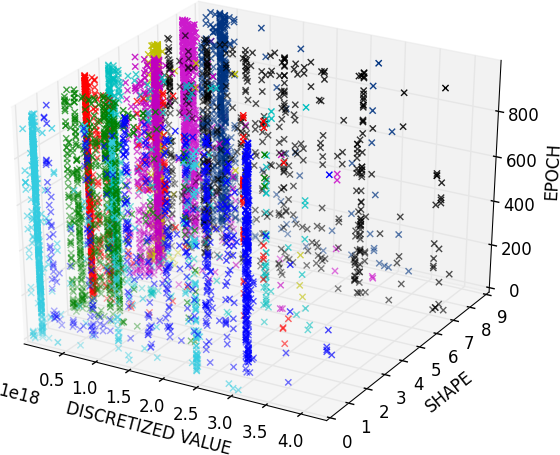
\includegraphics[width=250px]{data/expA3/discretize_cloud.png}
	  &
	  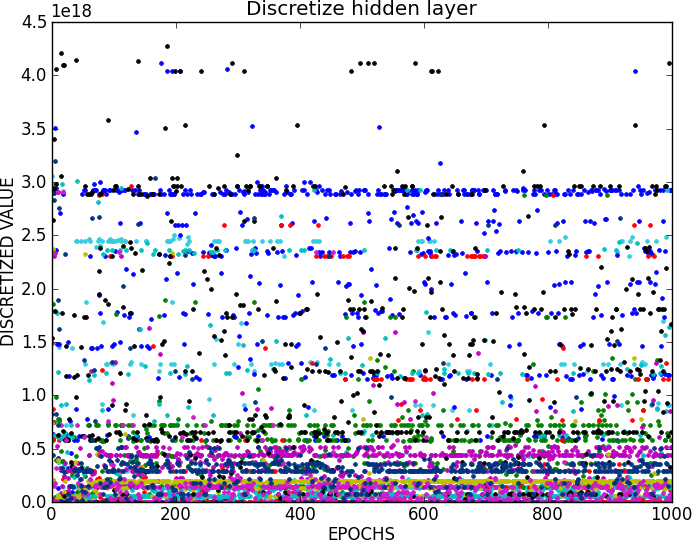
\includegraphics[width=250px]{data/expA3/discretize.png} 
	\end{tabular}
      \end{center} 
      \subparagraph{Notes}
	\begin{itemize}
	  \item une couleur équivaut à un chiffre présenté
	  \item une valeur discretisée correspond à un certain encodage de la couche cachée (cf Algorithmes~\nameref{discretize})
	\end{itemize}
      \subparagraph{Conclusion}
	Nous pouvons maintenant expliquer les raisons provoquant le mauvais apprentissage des entrées par le second réseau :
	
	Pour un seul chiffre présenté, il existe différentes valeurs de la couche cachée le représentant ( factorisation 
	dans la couche cachée du premier réseau). Le second réseau ne peut donc pas apprendre toutes les entrées.
	
	Une même valeur discretisée peut correspondre à plusieurs couleurs (différents nombres) ce qui augmentent la 
	difficulté d'apprentissage.
    \paragraph{Secondaires}
      Représentations au travers des poids du premier réseau
      \begin{center}
	Couche cachée \\
	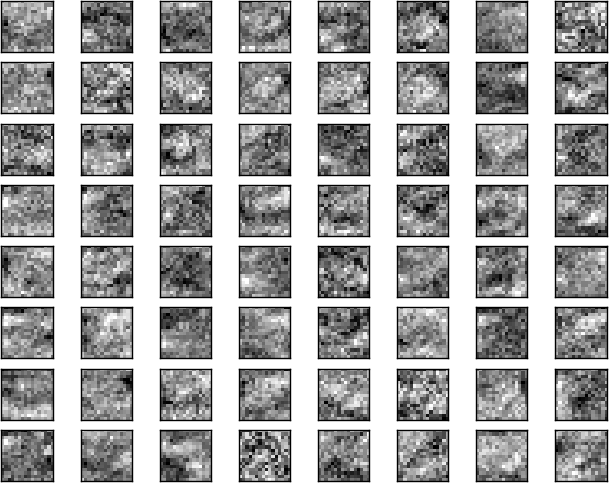
\includegraphics[width=250px]{data/expA3/representation_hidden.png}
      \end{center}
      \begin{center}
	Couche de sortie \\
	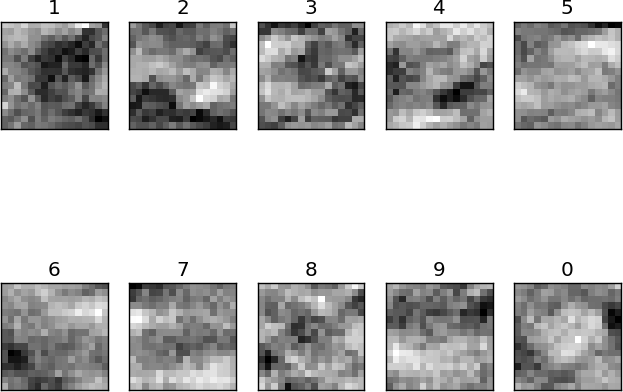
\includegraphics[width=250px]{data/expA3/representation.png}
      \end{center} 
      \subparagraph{Notes}
	\begin{itemize}
	  \item plus une case est noire, plus sa présence est importante pour le chiffre en question
	  \item plus une case est blanche, plus son absence est importante
	\end{itemize}
      \subparagraph{Conclusion}
	On arrive, sans trop de mal, à distinguer les chiffres.
    \paragraph{Secondaires}
      Prototypes à l'intérieur de la première partie de la couche de sortie du second réseau
      \begin{center}
	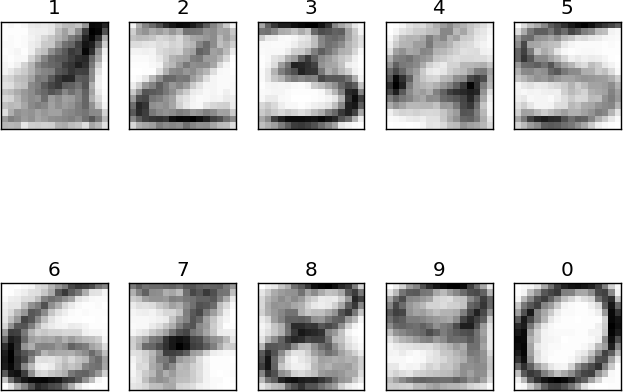
\includegraphics[width=250px]{data/expA3/prototype.png}
      \end{center} 
      \subparagraph{Notes}
	\begin{itemize}
	  \item Il sagit de la moyenne des réponses du second réseaux sur toutes les entrées
	\end{itemize}
      \subparagraph{Conclusion}
	Il est intéressant de constaté que malgrès la difficulté de la tâche, ces prototypes émergent.
	
	Et que contrairement à ce qu'indique les performances, les chiffres sont bien distincts.
      
	On peut, par ailleurs, conjecturer que plus la couche cachée du premier réseau est petite, plus les prototypes 
	seront factorisés (ie. personnels au réseau).
	


  \subsection{Conclusion}
  
  

  \newpage 
  \subsection{Formules}
    \paragraph{RMS} \label{rms}
  Pour une époque $e$ :
  \begin{center}
    \begin{large}
    $ rms_{e} = \sqrt{ \frac{1}{n} \sum \limits_{i=1}^{n} 
    ( o_{i,e} - d_{i} )^2 } $
    \end{large}
  $ with \left\lbrace \begin{array}{lll} n : number\ of\ neurons\ on\ the\ output\ 
  layer\\o_{i,e} : value\ obtained\ for\ the\ i^{th}\ neuron\ at\ the\ e^{th}\ epoch\\d_{i} : 
  value\ desired \ for\ the\ i^{th}\ neuron\end{array} \right.$
  \end{center}
    \paragraph{Discrétisation} \label{discretize}
      Pour la couche cachée $hiddenNeuron$ de $n$ neurones, un neurone
      pouvant être encodé par $number\_cutting$ valeurs différentes :
      \begin{center}
	$\sum \limits_{i=0}^{n} number\_cutting^{i} \times cutting(hiddenNeuron[i]) $
      \end{center}
      \subparagraph{Exemple}
	$400 \gets [0 ; 0,25 ]\ [0 ; 0,25 ]\  [0,25 ; 0,5 ]\  [0,5 ; 0,75 ]\  [0,25 ; 0,5 ]$ \\
	\hspace*{2.70cm}
	$400 \gets 0\times4^0 +   0\times4^1  +   1\times4^2   +  2\times4^3   +   1 \times4^4$
    \paragraph{Descente de gradient} \cite{Touzet_1992} \\
  Construction de l'erreur : 
    \begin{center}
      $y_{i} = f'(a_i) \times ( d_i - x_i ) \ si\ i\ neurone\ de\ sortie $ \\
      $y_{i} = f'(a_i) \times \sum \limits_{k} ( w_{ki} \times y_k )\ si\ i\ neurone\ cache $
    \end{center}
  Mise à jour des poids :
    \begin{center}
      $w_{ij}(t+1) = w_{ij}(t) + learning\_rate \times y_{i} \times x_j + momentum \times 
      (w_{ij}(t) - w_{ij}(t-1) )$
    \end{center}
  Variables : 
    \begin{center}
      $\left\lbrace \begin{array}{lll} 
	f : fonction\ sigmoide \\
	x_i : valeur\ du\ neurone\ i\\
	d_i : valeur\ desire pour\ le\ neurone\ i\\
	a_i : somme\ pondere\ des\ poids\ du\ neurone\ i
      \end{array} \right.$
    \end{center}

\bibliographystyle{../pre-rapport/apalike}
\bibliography{../pre-rapport/biblio}
